We report the upper limits obtained using the data with the run number $>=170826$ ( referred to 
as the post-EPS data) in the 0 and 1 jet bins separating the 
same flavor ($ee/\mu\mu$) and opposite flavor ($e\mu$) final states.
The observed and expected upper limits corresponding to the post-EPS data are shown in 
Figure~\ref{fig:limits_posteps_cut}-\ref{fig:limits_posteps_shape} for cut-based and multivariate 
based analyeses respectively, with the results tabulated in 
Table~\ref{tab:limits_posteps_cut}-\ref{tab:limits_posteps_shape} respectively.

%%%%%%%%%%%%%%%%%%%%%%%%%%%%%%
\begin{figure}[!htbp]
\centering
\subfigure[]{
\centering
\label{subfig:0j_sf}
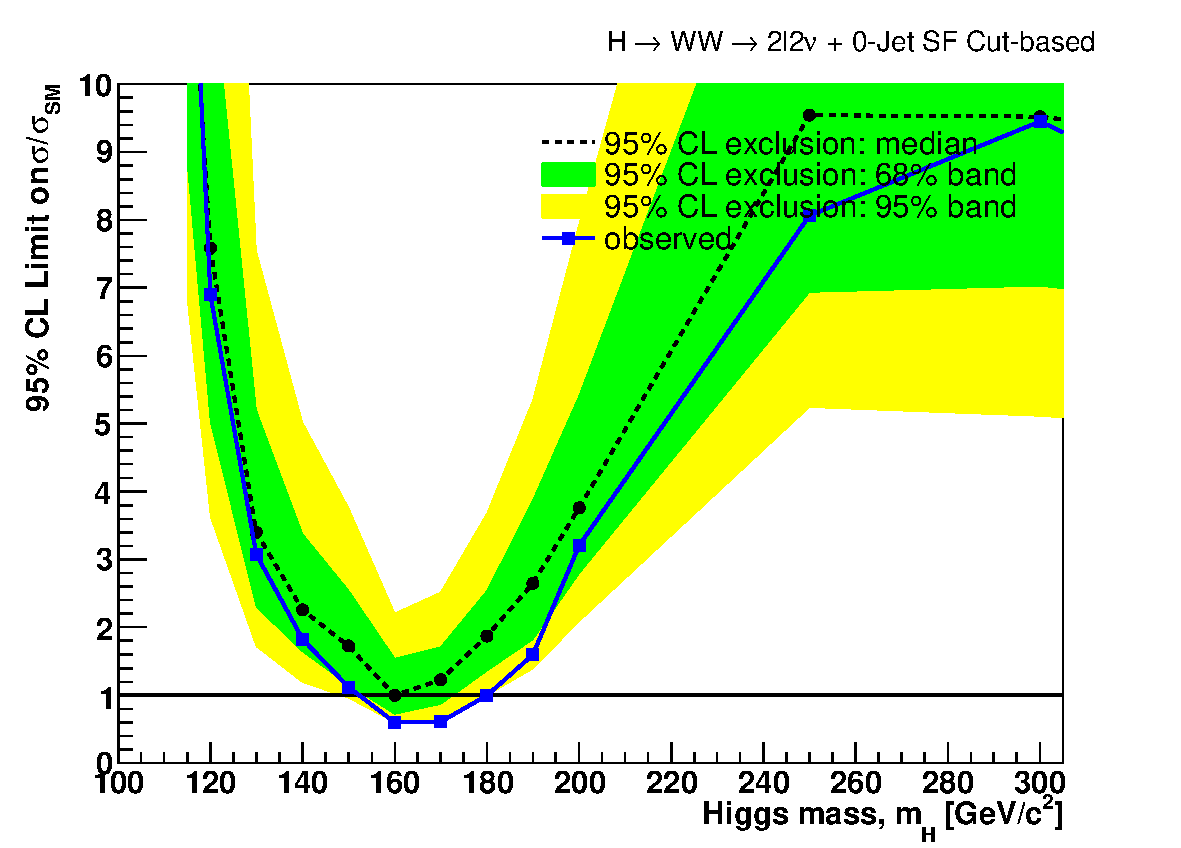
\includegraphics[width=0.48\textwidth]{lp_figures/limits_0j_sf_cut_ana_v6_1500pb_LP_POSTEPS.pdf}}
\subfigure[]{
\centering
\label{subfig:0j_of}
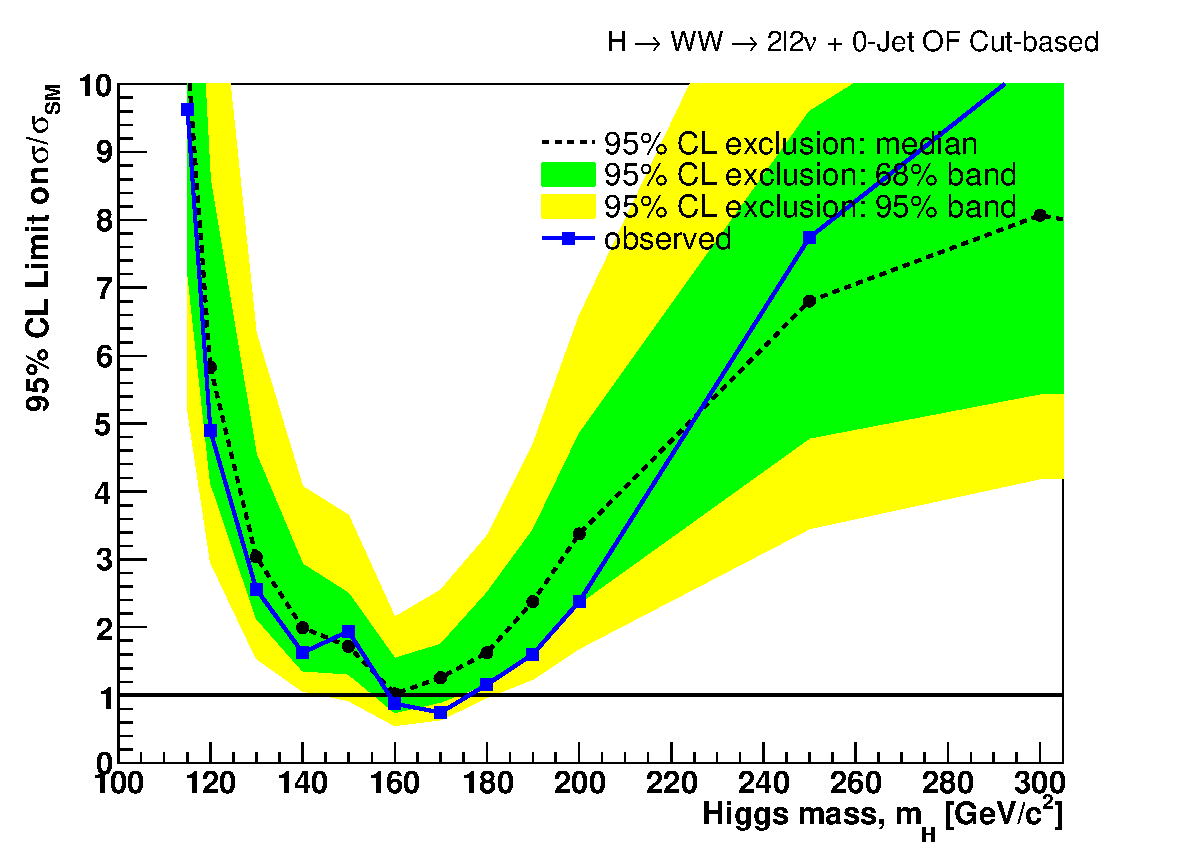
\includegraphics[width=0.48\textwidth]{lp_figures/limits_0j_of_cut_ana_v6_1500pb_LP_POSTEPS.pdf}}
\subfigure[]{
\centering
\label{subfig:1j_sf}
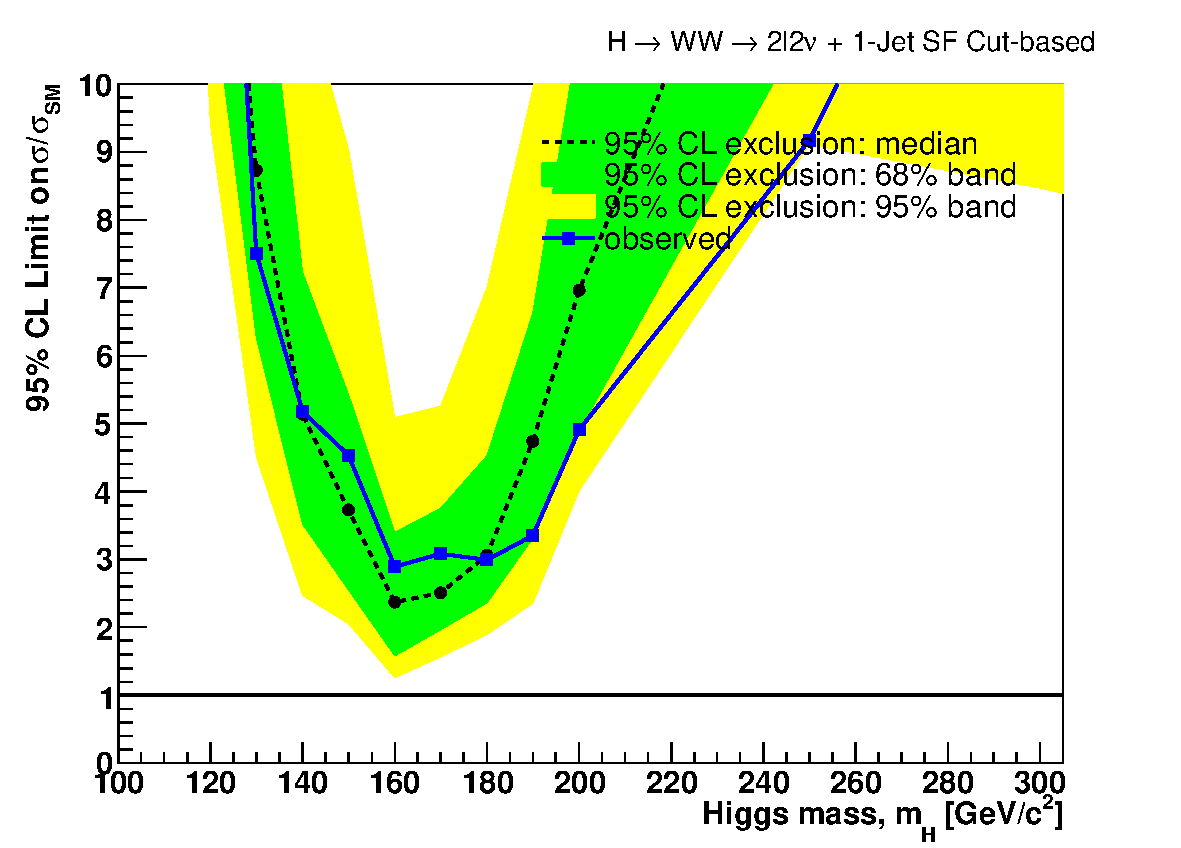
\includegraphics[width=0.48\textwidth]{lp_figures/limits_1j_sf_cut_ana_v6_1500pb_LP_POSTEPS.pdf}}
\subfigure[]{
\centering
\label{subfig:1j_of}
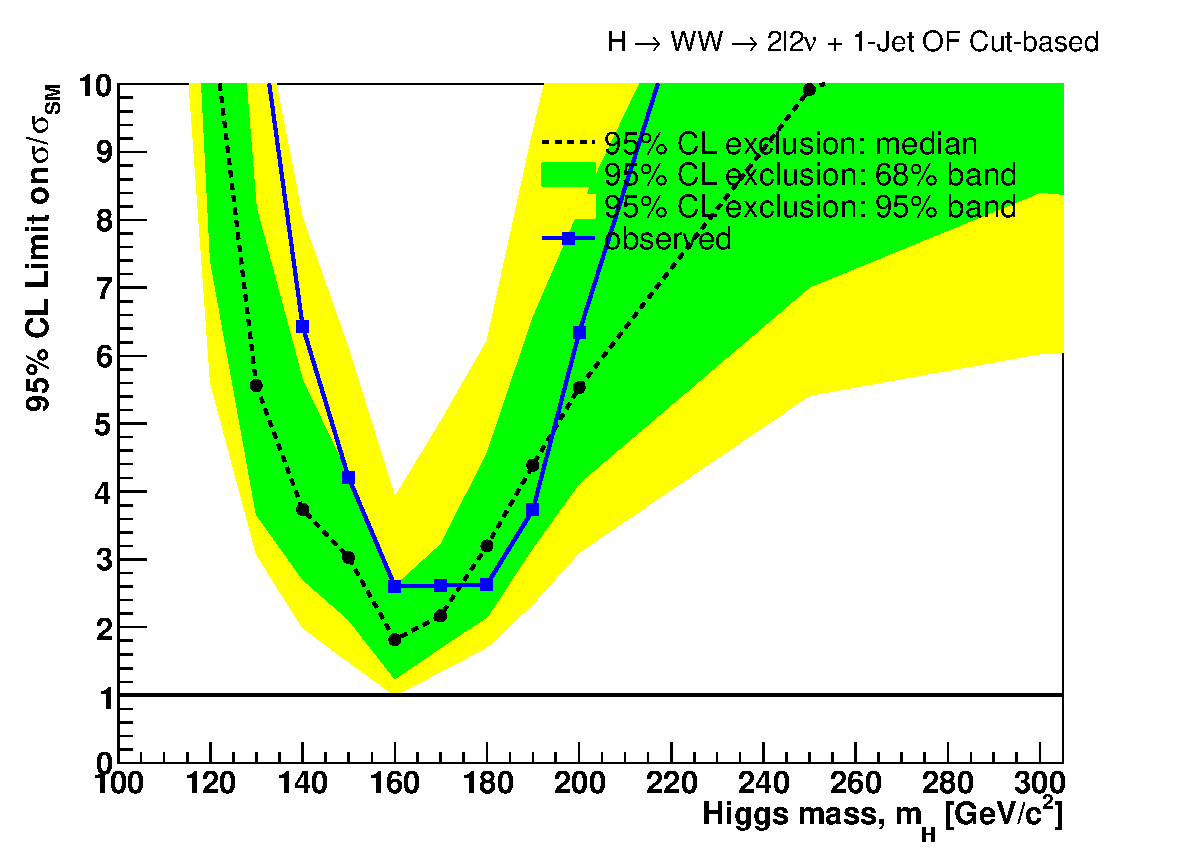
\includegraphics[width=0.48\textwidth]{lp_figures/limits_1j_of_cut_ana_v6_1500pb_LP_POSTEPS.pdf}}
\caption{Cut-based analysis upper limits at 95\% C.L. using the post-EPS data (run $>=$ 170826) corresponding to 0.4~$\ifb$.
The limits are shown in 4 final states separately. \subref{subfig:0j_sf}: SF in 0 Jet bin; 
\subref{subfig:0j_of}: OF in 0 Jet bin; \subref{subfig:1j_sf}: SF in 1 Jet bin; 
\subref{subfig:1j_of}: OF in 1 Jet bin; 
}
\label{fig:limits_posteps_cut}
\end{figure}
%%%%%%%%%%%%%%%%%%%%%%%%%%%%%%

%%%%%%%%%%%%%%%%%%%%%%%%%%%%%%
\begin{figure}[!htbp]
\centering
\subfigure[]{
\centering
\label{subfig:0j_sf}
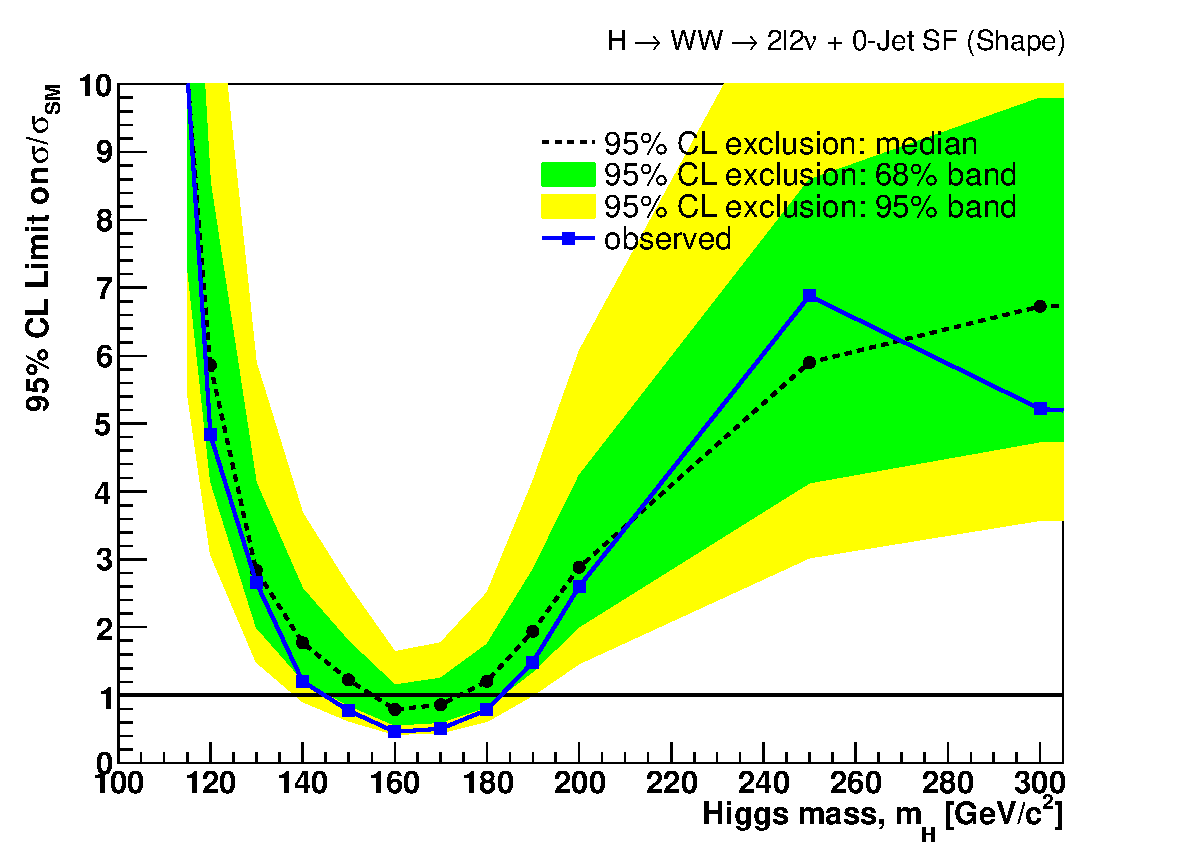
\includegraphics[width=0.48\textwidth]{lp_figures/limits_0j_sf_shape_ana_v6_1500pb_LP_POSTEPS.pdf}}
\subfigure[]{
\centering
\label{subfig:0j_of}
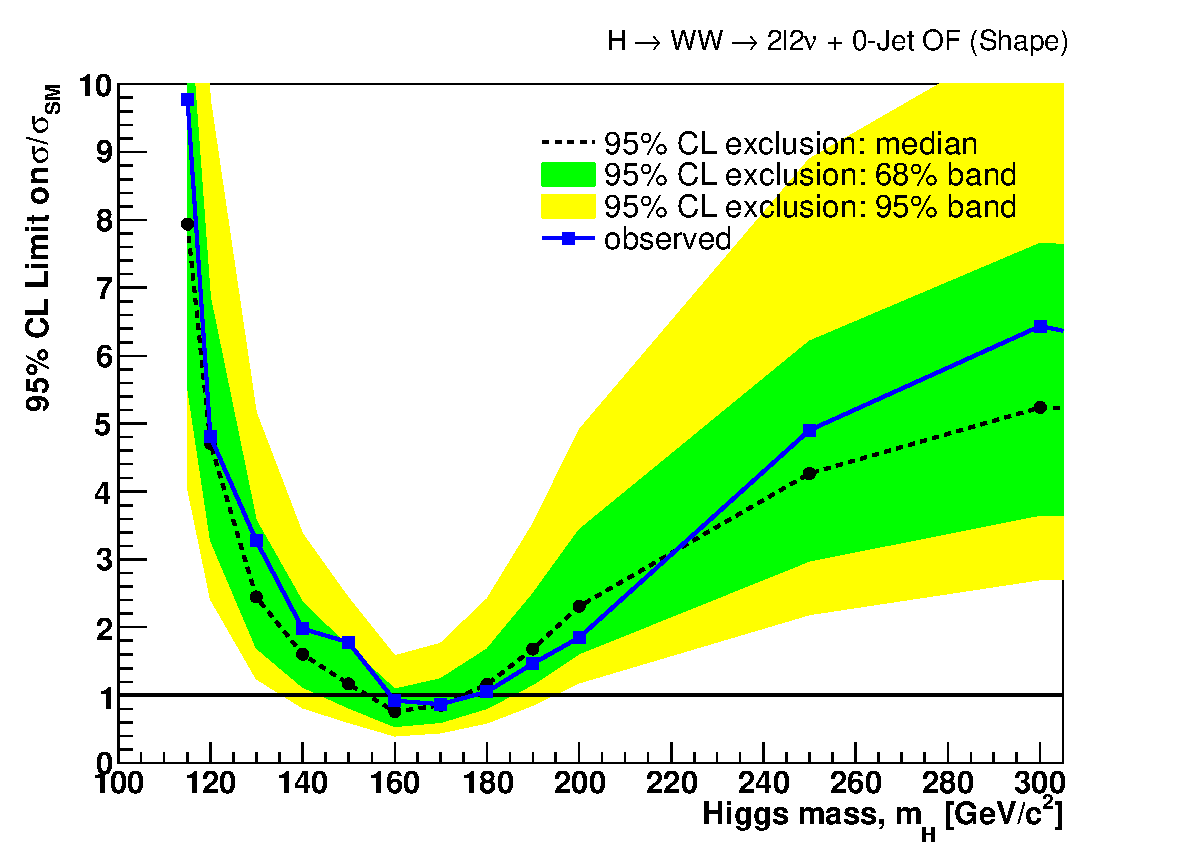
\includegraphics[width=0.48\textwidth]{lp_figures/limits_0j_of_shape_ana_v6_1500pb_LP_POSTEPS.pdf}}
\subfigure[]{
\centering
\label{subfig:1j_sf}
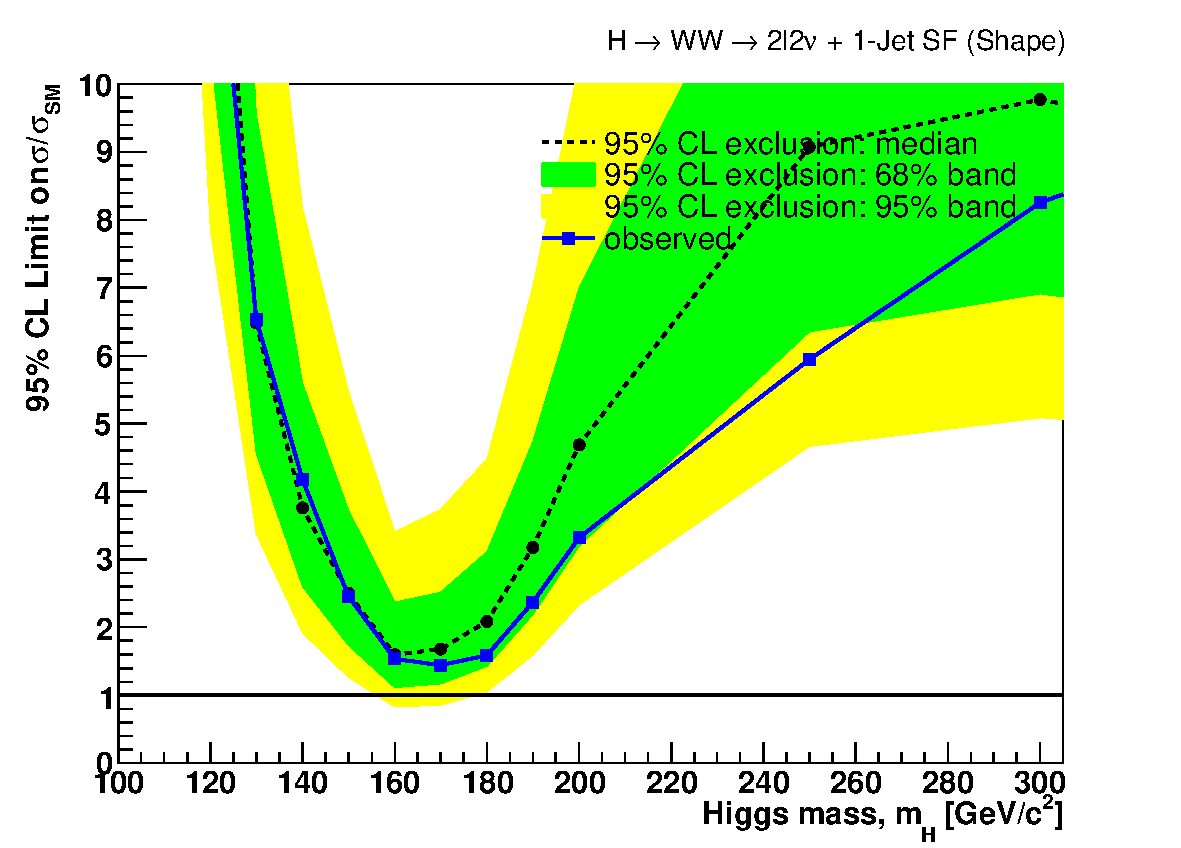
\includegraphics[width=0.48\textwidth]{lp_figures/limits_1j_sf_shape_ana_v6_1500pb_LP_POSTEPS.pdf}}
\subfigure[]{
\centering
\label{subfig:1j_of}
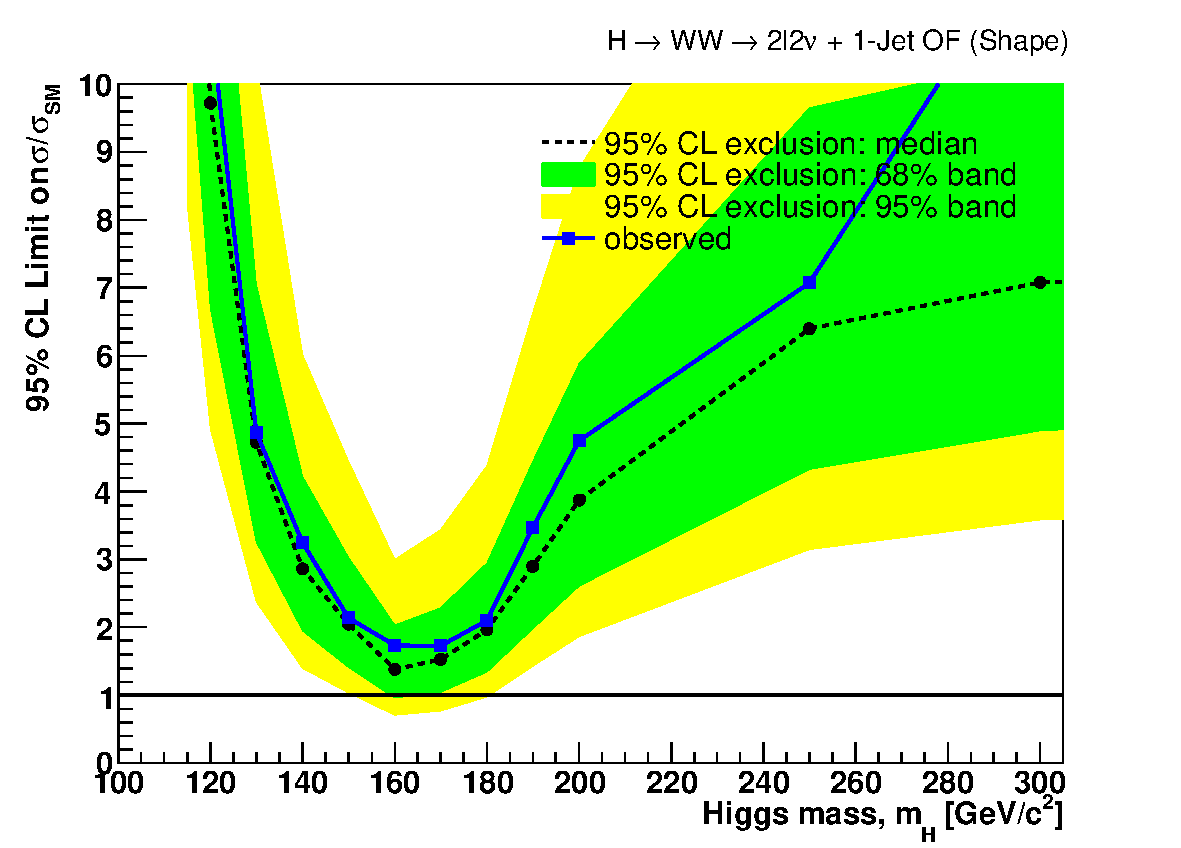
\includegraphics[width=0.48\textwidth]{lp_figures/limits_1j_of_shape_ana_v6_1500pb_LP_POSTEPS.pdf}}
\caption{Mutivariate based analysis upper limits at 95\% C.L. using the post-EPS data (run $>=$ 170826) corresponding to 0.4~$\ifb$.
The limits are shown in 4 final states separately. \subref{subfig:0j_sf}: SF in 0 Jet bin; 
\subref{subfig:0j_of}: OF in 0 Jet bin; \subref{subfig:1j_sf}: SF in 1 Jet bin; 
\subref{subfig:1j_of}: OF in 1 Jet bin; 
}
\label{fig:limits_posteps_shape}
\end{figure}
%%%%%%%%%%%%%%%%%%%%%%%%%%%%%%

%%%%%%%%%%%%%%%%%%%%%%%%%%%%%%
\begin{table}
\begin{center}
\begin{tabular}{c c c c c}
\hline\hline
 $m_H$ (GeV) & Observed & Median Expected & 68\% C.L. Band & 95\% C.L. Band \\ \hline
\hline
\multicolumn{5}{c} {0-Jet Bin Same Flavor} \\
\hline
115 & 14.3 & 12.9 & [8.8, 21.4] & [6.8, 43.3] \\
120 & 6.9 & 7.6 & [5.0, 11.9] & [3.6, 21.3] \\
130 & 3.1 & 3.4 & [2.3, 5.2] & [1.7, 7.5] \\
140 & 1.8 & 2.3 & [1.6, 3.4] & [1.2, 5.0] \\
150 & 1.1 & 1.7 & [1.1, 2.5] & [1.0, 3.8] \\
160 & 0.6 & 1.0 & [0.7, 1.5] & [0.6, 2.2] \\
170 & 0.6 & 1.2 & [0.9, 1.7] & [0.6, 2.5] \\
180 & 1.0 & 1.9 & [1.4, 2.5] & [1.0, 3.7] \\
190 & 1.6 & 2.6 & [1.8, 3.9] & [1.4, 5.3] \\
200 & 3.2 & 3.8 & [2.8, 5.4] & [2.1, 7.9] \\
250 & 8.1 & 9.5 & [6.9, 14.4] & [5.2, 20.2] \\
300 & 9.5 & 9.5 & [7.0, 14.4] & [5.1, 20.2] \\
\hline
\multicolumn{5}{c} {0-Jet Bin Opposite Flavor} \\
\hline
115 & 9.6 & 10.4 & [7.2, 15.1] & [5.2, 22.3] \\
120 & 4.9 & 5.8 & [4.1, 8.6] & [3.0, 12.8] \\
130 & 2.6 & 3.0 & [2.1, 4.5] & [1.5, 6.3] \\
140 & 1.6 & 2.0 & [1.4, 2.9] & [1.1, 4.1] \\
150 & 1.9 & 1.7 & [1.3, 2.5] & [0.9, 3.7] \\
160 & 0.9 & 1.0 & [0.7, 1.5] & [0.6, 2.2] \\
170 & 0.7 & 1.3 & [0.9, 1.7] & [0.6, 2.6] \\
180 & 1.2 & 1.6 & [1.2, 2.5] & [1.0, 3.3] \\
190 & 1.6 & 2.4 & [1.6, 3.4] & [1.2, 4.7] \\
200 & 2.4 & 3.4 & [2.4, 4.8] & [1.7, 6.6] \\
250 & 7.7 & 6.8 & [4.8, 9.6] & [3.5, 13.7] \\
300 & 10.4 & 8.1 & [5.4, 11.7] & [4.2, 16.0] \\
\hline
\multicolumn{5}{c} {1-Jet Bin Same Flavor} \\
\hline
115 & 37.5 & 31.2 & [21.4, 50.3] & [17.2, 74.9] \\
120 & 19.1 & 16.3 & [11.7, 25.6] & [9.4, 42.9] \\
130 & 7.5 & 8.7 & [6.3, 13.2] & [4.5, 21.9] \\
140 & 5.2 & 5.1 & [3.5, 7.2] & [2.5, 11.4] \\
150 & 4.5 & 3.7 & [2.6, 5.4] & [2.1, 9.0] \\
160 & 2.9 & 2.4 & [1.6, 3.4] & [1.3, 5.1] \\
170 & 3.1 & 2.5 & [2.0, 3.8] & [1.6, 5.3] \\
180 & 3.0 & 3.1 & [2.4, 4.5] & [1.9, 7.0] \\
190 & 3.3 & 4.7 & [3.3, 6.6] & [2.4, 9.9] \\
200 & 4.9 & 7.0 & [4.9, 10.8] & [4.0, 15.4] \\
250 & 9.2 & 15.3 & [11.0, 23.8] & [9.1, 34.2] \\
300 & 16.0 & 15.9 & [11.5, 21.6] & [8.5, 30.9] \\
\hline
\multicolumn{5}{c} {1-Jet Bin Opposite Flavor} \\
\hline
115 & 41.3 & 19.6 & [14.2, 29.5] & [10.4, 41.5] \\
120 & 24.8 & 11.2 & [7.4, 16.5] & [5.6, 24.4] \\
130 & 11.4 & 5.6 & [3.7, 8.2] & [3.1, 11.5] \\
140 & 6.4 & 3.7 & [2.7, 5.6] & [2.0, 8.0] \\
150 & 4.2 & 3.0 & [2.1, 4.2] & [1.5, 6.1] \\
160 & 2.6 & 1.8 & [1.2, 2.6] & [1.0, 3.9] \\
170 & 2.6 & 2.2 & [1.7, 3.2] & [1.4, 5.0] \\
180 & 2.6 & 3.2 & [2.2, 4.6] & [1.7, 6.2] \\
190 & 3.7 & 4.4 & [3.2, 6.6] & [2.4, 9.3] \\
200 & 6.3 & 5.5 & [4.1, 8.1] & [3.1, 12.2] \\
250 & 17.0 & 9.9 & [7.0, 15.2] & [5.4, 21.8] \\
300 & 21.4 & 11.2 & [8.4, 17.3] & [6.0, 24.9] \\
\hline\hline
\end{tabular}
\end{center}
\caption{Cut-based upper limits at 95\% C.L. in 0 and 1 Jet final state, 
using the post-EPS data (run $>=$ 170826) corresponding to  0.4~$\ifb$ 
shown in Figure~\ref{fig:limits_posteps_cut}.}
\label{tab:limits_posteps_cut}
\end{table}
%%%%%%%%%%%%%%%%%%%%%%%%%%%%%%




%%%%%%%%%%%%%%%%%%%%%%%%%%%%%%
\begin{table}
\begin{center}
\begin{tabular}{c c c c c}
\hline\hline
 $m_H$ (GeV) & Observed & Median Expected & 68\% C.L. Band & 95\% C.L. Band \\ \hline
\hline
\multicolumn{5}{c} {0-Jet Bin Same Flavor} \\
\hline
115 & 10.2 & 10.2 & [7.3, 14.7] & [5.4, 20.9] \\
120 & 4.8 & 5.9 & [4.2, 8.5] & [3.1, 12.4] \\
130 & 2.7 & 2.8 & [2.0, 4.1] & [1.5, 5.9] \\
140 & 1.2 & 1.8 & [1.2, 2.6] & [0.9, 3.7] \\
150 & 0.8 & 1.2 & [0.9, 1.8] & [0.6, 2.6] \\
160 & 0.5 & 0.8 & [0.6, 1.1] & [0.4, 1.6] \\
170 & 0.5 & 0.9 & [0.6, 1.2] & [0.4, 1.8] \\
180 & 0.8 & 1.2 & [0.8, 1.8] & [0.6, 2.5] \\
190 & 1.5 & 1.9 & [1.3, 2.8] & [1.0, 4.1] \\
200 & 2.6 & 2.9 & [2.0, 4.2] & [1.5, 6.1] \\
250 & 6.9 & 5.9 & [4.1, 8.6] & [3.0, 12.3] \\
300 & 5.2 & 6.7 & [4.7, 9.8] & [3.6, 14.0] \\
\hline
\multicolumn{5}{c} {0-Jet Bin Opposite Flavor} \\
\hline
115 & 9.8 & 7.9 & [5.5, 11.5] & [4.1, 16.5] \\
120 & 4.8 & 4.7 & [3.3, 6.9] & [2.4, 9.8] \\
130 & 3.3 & 2.4 & [1.7, 3.6] & [1.2, 5.2] \\
140 & 2.0 & 1.6 & [1.1, 2.4] & [0.8, 3.4] \\
150 & 1.8 & 1.2 & [0.8, 1.7] & [0.6, 2.4] \\
160 & 0.9 & 0.8 & [0.5, 1.1] & [0.4, 1.6] \\
170 & 0.9 & 0.9 & [0.6, 1.2] & [0.4, 1.8] \\
180 & 1.0 & 1.2 & [0.8, 1.7] & [0.6, 2.4] \\
190 & 1.5 & 1.7 & [1.2, 2.5] & [0.8, 3.5] \\
200 & 1.9 & 2.3 & [1.6, 3.4] & [1.2, 4.9] \\
250 & 4.9 & 4.3 & [3.0, 6.2] & [2.2, 8.9] \\
300 & 6.4 & 5.2 & [3.7, 7.7] & [2.7, 10.9] \\
\hline
\multicolumn{5}{c} {1-Jet Bin Same Flavor} \\
\hline
115 & 26.5 & 26.2 & [18.5, 38.7] & [14.1, 55.0] \\
120 & 13.4 & 15.0 & [10.5, 22.0] & [7.9, 32.3] \\
130 & 6.5 & 6.5 & [4.6, 9.6] & [3.4, 13.9] \\
140 & 4.2 & 3.8 & [2.6, 5.6] & [1.9, 8.2] \\
150 & 2.5 & 2.5 & [1.7, 3.7] & [1.3, 5.5] \\
160 & 1.5 & 1.6 & [1.1, 2.4] & [0.8, 3.4] \\
170 & 1.4 & 1.7 & [1.2, 2.5] & [0.9, 3.7] \\
180 & 1.6 & 2.1 & [1.4, 3.1] & [1.0, 4.5] \\
190 & 2.4 & 3.2 & [2.2, 4.7] & [1.6, 7.0] \\
200 & 3.3 & 4.7 & [3.2, 7.0] & [2.3, 10.3] \\
250 & 5.9 & 9.1 & [6.3, 13.6] & [4.7, 19.9] \\
300 & 8.3 & 9.8 & [6.9, 14.4] & [5.1, 20.9] \\
\hline
\multicolumn{5}{c} {1-Jet Bin Opposite Flavor} \\
\hline
115 & 20.2 & 15.9 & [11.1, 23.5] & [8.2, 33.6] \\
120 & 11.0 & 9.7 & [6.7, 14.3] & [4.9, 20.9] \\
130 & 4.9 & 4.7 & [3.3, 7.1] & [2.4, 10.3] \\
140 & 3.2 & 2.9 & [2.0, 4.2] & [1.4, 6.0] \\
150 & 2.1 & 2.0 & [1.4, 3.0] & [1.0, 4.4] \\
160 & 1.7 & 1.4 & [1.0, 2.0] & [0.7, 3.0] \\
170 & 1.7 & 1.5 & [1.0, 2.3] & [0.8, 3.4] \\
180 & 2.1 & 2.0 & [1.3, 2.9] & [1.0, 4.4] \\
190 & 3.5 & 2.9 & [2.0, 4.4] & [1.4, 6.6] \\
200 & 4.7 & 3.9 & [2.6, 5.9] & [1.9, 8.8] \\
250 & 7.1 & 6.4 & [4.3, 9.6] & [3.1, 14.1] \\
300 & 12.3 & 7.1 & [4.9, 10.4] & [3.6, 15.4] \\
\hline\hline
\end{tabular}
\end{center}
\caption{Multivariate based upper limits at 95\% C.L. in 0 and 1 Jet final state, 
using the post-EPS data (run $>=$ 170826) corresponding to  0.4~$\ifb$ 
shown in Figure~\ref{fig:limits_posteps_shape}.}
\label{tab:limits_posteps_shape}
\end{table}
%%%%%%%%%%%%%%%%%%%%%%%%%%%%%%

